\documentclass[a4paper,11pt]{book}
\usepackage{graphicx}
\usepackage{hyperref}
\usepackage[utf8]{inputenc}
\usepackage{texnames}
\usepackage{amsmath}
\usepackage[T1]{fontenc}
\pagestyle{plain}
\usepackage{multicol}
\usepackage{color}
\usepackage{cancel}
\usepackage{caption}
\usepackage{subcaption}
\usepackage[margin=0.5in]{geometry}

\title{BPMs Positioning System Operation}
\author{Oscar BLANCO}
\date{\today}

\graphicspath{{./figures/}}

\begin{document}
\maketitle
\tableofcontents
\frontmatter
\chapter{Introduction}
\mainmatter
\chapter{Status}
\section{Linearity}
\begin{figure}
\centering
 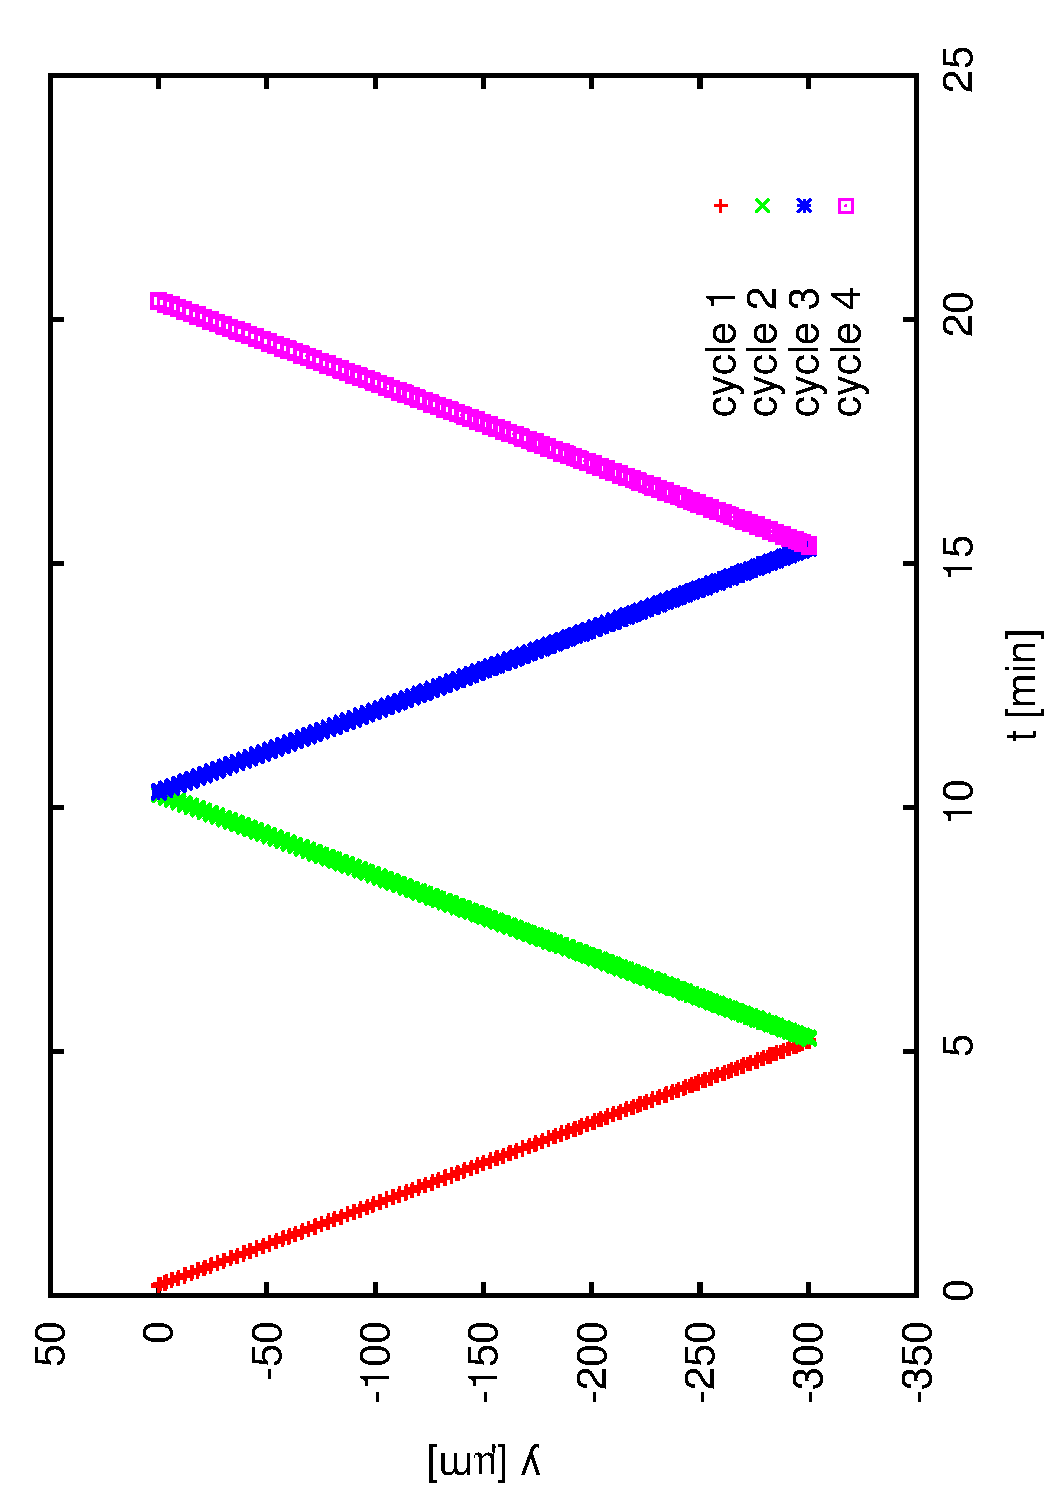
\includegraphics[scale=0.5,angle=-90]{image01.pdf}\caption{PI movers linearity}\label{f-LinPI01}
\end{figure}
\section{Coupling}
\begin{figure}
\centering
 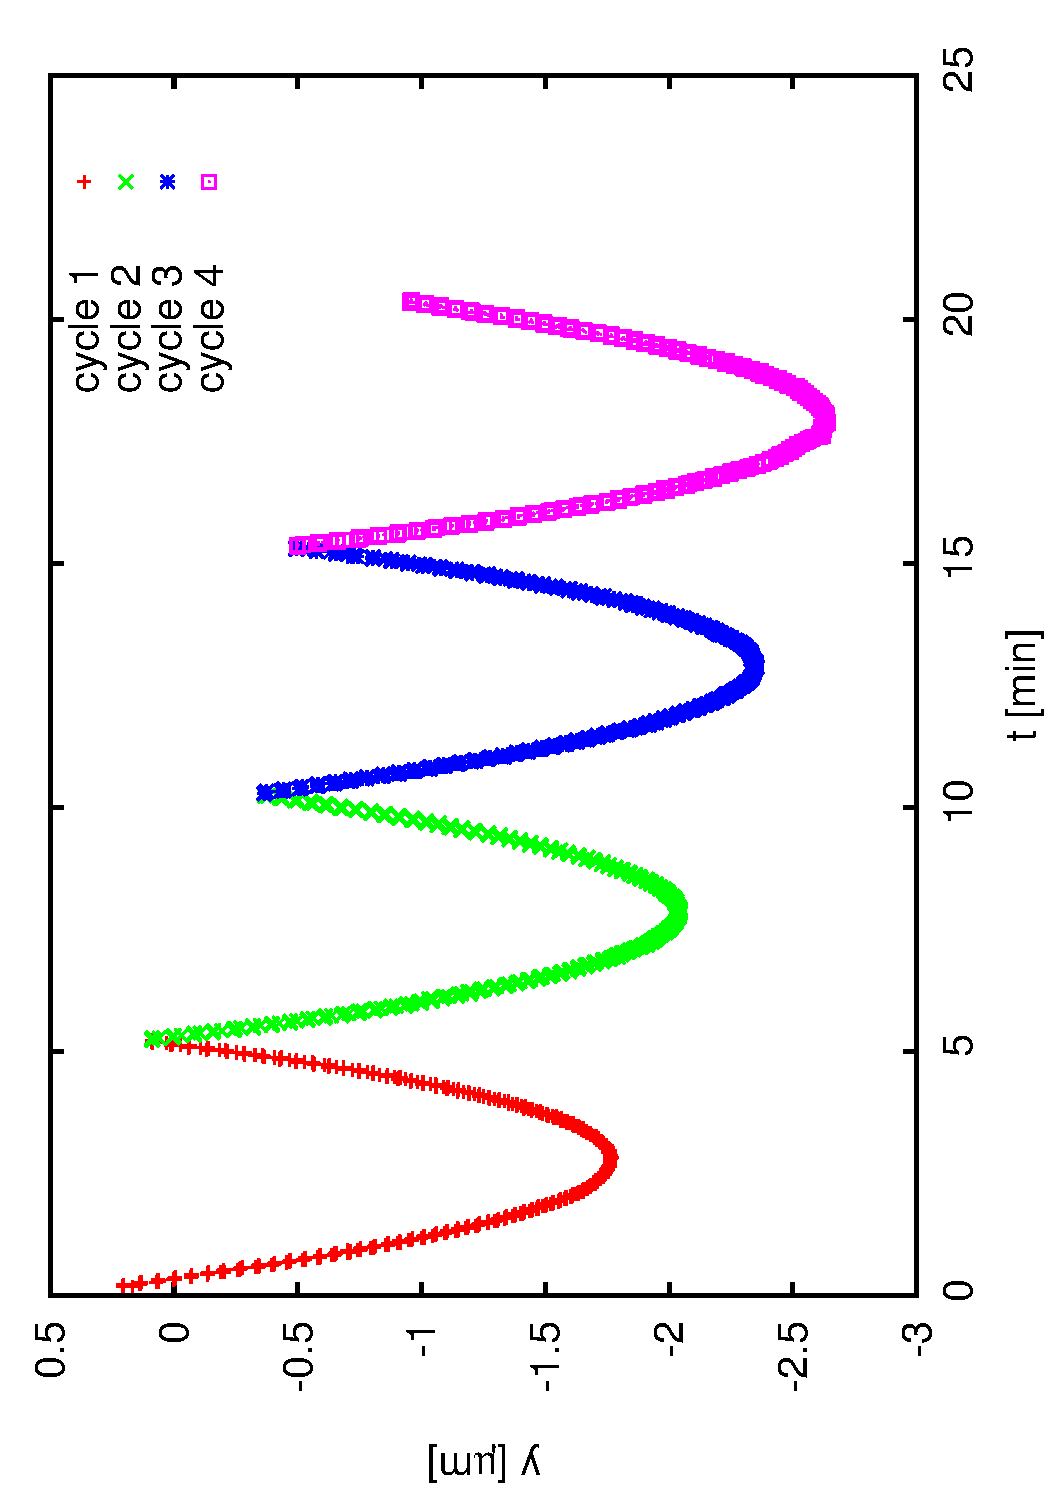
\includegraphics[scale=0.5,angle=-90]{image41.pdf}\caption{PI movers coupling}\label{f-LinPI41}
\end{figure}

\appendix
\chapter{Appendix}
\section{Document sources}
\url{https://github.com/orblancog/ATF2_IPBPMmovers_user_manual}
\backmatter
\chapter{Discussion, conclusions}
\listoffigures
\listoftables
ATF2 - KEK


Release: 04
Date: 30/07/2013


Introduction

System Description
At the ATF2 IP, inside the vacuum chamber, the BPMs positioning system has been installed during the first two weeks of July 2013.
It will move two blocks: 
BPMs 1 2
BPM 3
This movement has two degrees of freedom: vertical (y) and lateral (x), both transverse to the beam direction. Beam crosses BPM12 first, then and empty space where Shintake monitor laser will be aligned, then crosses BPM3 and goes out of the vacuum chamber.

These two blocks of BPMs, moving in two directions each, are displaced by Piezo-Movers (or just movers) made by different companies. German «PI electronics« moves  BPM3 and French «Cedrat Technologies« moves BPM12.

Each block has 3 vertical and one lateral movers. Lateral is underneath. Four movers are used per block, eight in total.

The Piezo Movers

Piezo mover changes its position as a function of voltage. Each one of the eight movers has its own control electronics block composed of: 
the mover
the strain gauge
manufacturer module to:
set piezo mover voltage (high voltage)
PI module E-621
CEDRAT module LA75
read strain gauge
PI module E-621 (same as control)
CEDRAT module SG75
set feedback operation (ON/OFF)
set control mode (external control from PLC is used)
PLC channel to
set control voltage values equivalent to piezo mover displacement
read voltage values equivalent to strain gauge deformation

PI and Cedrat have different ranges:
PI (300um), Cedrat (250um)

Control voltage and its relation with displacement (min-max) varies between both companies:
PI: 		(min)   0V   	to 	(max) 10V
CEDRAT: 	(max) -1V 	to	(min)    7V
It is important to note that:
The voltage-displacement relation is inverse for CEDRAT movers.
When the system is OFF (0V), PI mover are at its minimum, however CEDRAT are not.

Feedback and NO Feedback 
There are two operation possibilitiesper mover: Feedback (fb) and No Feedback (no fb). It means 8 feedback loops. On each case the control module sets a voltage value on the mover and read the strain gauge to create a closed loop. However, their implementations are different on each company.

PI has an analogue feedback system adjusted to the best possible performance on an individual mover (avoid piezo-mover channel interchange). Do not exchange fb/no fb while the equipment is ON. Turn it OFF before any modification. 
Feedback is controlled by the switch number 3  on the front panel. 
Feedback ON (left) / Feedback OFF (right)
During operation, when feedback is ON and working properly two green LED are on (Power LED, On Target LED). When no feedback just the Power LED is green.

Cedrat has a digital feedback system with PID parameters per mover. Avoid piezo-mover channel interchange. Feedback could be turn off/on by two means:
Switch SERVO ON in the front pannel. Feedback ON(right)/Feedback OFF (left)
Using sofware  HDPM45V16. To activate or desactivate permanently the fb.

The PLC

Two NI9263 are used to set analogue voltage into the mover control electronics.
Two NI9239 are used to read analogue voltage from the strain gauge readback.
One NI9219 is used to read temperature.
These modules are connected to the chassis NI9188 which is connected by network to a working station with Labview installed.
The block chassis+NI modules is called PLC.

- National instruments Chassis: NI9188
Mac Address: 0080.2f14.b777
DHCP
IP address (ATF) 31.1.1.39
IP address (KEK): None
Host name: ipmv-plc.ip-local
Net Mask: 255.255.255.0
connected to ip-local during installation
Chassis NI9188 can connect up to 8 modules, not all are used:
PI
Module 5: NI9263 Digital to analogue converter
Module 6: NI9239 Analogue to digital converter
Cedrat
Module 2: NI9263 Digital to analogue converter
Module 3: NI9239 Analogue to digital converter
Temperature
Module 8: NI9219 Temperature probes
Cedrat: 	Channel 0
PI: 		Channel 2

The PC
It is used to control from close locations the BPM positioning system. It sets the digital values to put in the PLC and reads the digital values from the PLC channels corresponding to strain gauges.

Used Software
Windows 7 Français
National Instrument - Labview 2011
National Instruments - Measurement $\&$s Automation Explorer (NI MAX)
Gimp 2.8
Microsoft office – Excel 2013
cmd
Highly Dynamic and Precise motion 45 V 1.6 (HDPM45V16)– Cedrat Technologies
LAL Computer (Laptop)
Account: atf2 admin
Password: KEKJapan2012
Processor Inter Core i7 vPro
Mac Address: d067.e550.620e
DHCP
IP address(ATF): 31.1.1.38
IP address (KEK): Wifi connection (MAC registered at KEK)
Net Mask: 255.255.255.0
connected to ip-local during installation
Folder Content description
Path to applications and info
		    Bureau/Actionneurs Piezo/Applis
All applications were done in Labview. Title gives a hint of its content:
	(keywords used in titles):
oscilloscope: uses de ADC to read signals
generateur: function generator, uses de DACs to produce signals
Actionneurs positionnement BPMs: activate the system displacement
Ethernet: connected by wired network,
USB: corresponds to previous version connected by USB.
Verticaux groupe: all 3 vertical mover movers are activated by one voltage control
 mouvements identiques: first version of BPM displacement system (PI and CEDRAT) integrated.
Jauges: stores the strain gauges info in excel format.
temp: stores temperature info in excel format.
epics: control from epics system, Labview works as interface.
Actionneurs multicycles: several cycles over the defined voltage range are performed
Cedrat, PI: identifies the group of movers to use.
Vertical, lateral fixe: it means that one direction of movement is set (fixed) to a voltage value while the other direction varies in cycles.


Quick start

Initialize the system
1. If any cable is hanging disconnected, first verify where it should be. All cables should be connected
2. Verify that PC and PLC are connected to network. During installation, both were connected to a hub and this was connected to ip-local.
3. PLC has no switch, it starts to work as soon it is connected and power is stable. If not connected, do this first. An orange LED will turn off when ready.
4. Cedrat has two ON switches. One in the back (main) and one in the front (connect and disconnects all input/outputs).
PI has one ON switch in the back.
PC (Laptop) has a switch on the front after opening the screen.
These three can be turn on in any order.
5. Let PI and Cedrat control electronics to heat up for 10 mins if first use during the day.
6. If the computer went to sleep or it is the first time in the day. It will be necessary to reinitialize the PLC. Follow these instructions.
1. Open the «National Instruments - Measurement \& Automation Explorer NI MAX«.
2. Select Périphériques et Interfaces
3. select Périphériques réseau.
4. If it is recognized, right-click over the peripheric and select «Réinitialiser le châssis«. A success prompt will appear some seconds after.
7. Open any of the previous programs designed in Labview to operate the system. Some of them can store the info in Excel format.
1. EPICS: if you are using EPICS, use the application:
"Bureau/Actionneurs Piezo/Applis Actionneurs positionnement BPMs - Ethernet - epics.vi" 
2. Local system: use any of the avalaible applications

Shut down
1. Close all programs
2. Shut down PC, Cedrat and PI control electronics in any order.
PLC is left ON.
How to acquire data
When logged at atf-user.atf-local server, do:
To set voltage value:
Remember to use a PV which ends in Write.
Using one which ends in Read has no effect
\$ caput PVname Value
To get voltage from strain gauges:
Remember to use a PV which ends in Read.
Using one which ends in Write has no effect
\$ caget PVname
\$ camonitor Pvname (or PVnames)

NOTES
Epics PVs (Process Variables)
Write: sets a value on the DAC.
Read: reads from ADC.
Channels IP:BPM-AB:Mover0 and IP:BPM-C:MoverB are for lateral movement.

IP:BPM-AB:Mover0:Read
IP:BPM-AB:Mover0:Write
IP:BPM-AB:Mover1:Read
IP:BPM-AB:Mover1:Write
IP:BPM-AB:Mover2:Read
IP:BPM-AB:Mover2:Write
IP:BPM-AB:Mover3:Read
IP:BPM-AB:Mover3:Write

IP:BPM-C:MoverB:Read
IP:BPM-C:MoverB:Write
IP:BPM-C:MoverC:Read
IP:BPM-C:MoverC:Write
IP:BPM-C:MoverD:Read
IP:BPM-C:MoverD:Write
IP:BPM-C:MoverE:Read
IP:BPM-C:MoverE:Write

IP:BPM-AB:Temp
IP:BPM-C:Temp
Older Epics PVs, DO NOT USE (Process Variables)
These PVs are here for documentation purposes. They are still functional but any new work should be done with previously defined PV in this document.
Write: sets a value on the DAC.
Read: reads from ADC.
Channels Cedrat0 and PIB are for lateral movement.

IPBSM:BPMs:PIB:Write
IPBSM:BPMs:PIB:Read
IPBSM:BPMs:PIC:Write
IPBSM:BPMs:PIC:Read
IPBSM:BPMs:PID:Write
IPBSM:BPMs:PID:Read
IPBSM:BPMs:PIE:Write
IPBSM:BPMs:PIE:Read


IPBSM:BPMs:Cedrat0:Write
IPBSM:BPMs:Cedrat0:Read
IPBSM:BPMs:Cedrat1:Write
IPBSM:BPMs:Cedrat1:Read
IPBSM:BPMs:Cedrat2:Write
IPBSM:BPMs:Cedrat2:Read
IPBSM:BPMs:Cedrat3:Write
IPBSM:BPMs:Cedrat3:Read

Read temperature:
IPBSM:BPMs:Temp1
IPBSM:BPMs:Temp2

Q/A and Troubleshooting
Is there any connection problem with the chassis?
A1: Check voltage and network cable connection. If status led is in orange it stills need sometime to operate.
A2: Open the «National Instruments - Measurement \& Automation Explorer NI MAX«. Select Périphériques et Interfaces, select Périphériques réseau. If it is recognized, right-click over the peripheric and select «Réinitialiser le châssis«. A success prompt will appear some seconds after.
A3: If the ni9188 appears, but you are not able to set (unset) parameters. Push the reset button in the chassis for at least 5 seconds. It will set all parameters to default.
A4: If you still have problems, disconnect all cables for at least 10 seconds and reconnect.
A5: If required the PLC can connect directly with the PC via network cable (no crossing). Reset all parameters and reconnect.

Are values at the readback different from the voltage set?
A1: it is normal to have a difference up to milivolts. Difference might be larger at the extreme points in PI and in the middle range for CEDRAT.
A2: If difference is larger, it is possible that feedback system is not connected. In doubt  consult the corresponding manual.
A3: Normally all front lights in PI and CEDRAT system should be green. If not, there is a electrical problem. Most common situation is that something is disconnected. Labels have been placed per cable in order to easily identify where does it belongs.
A4: Check power voltage and compare with the operation ranges at the back of PI and CEDRAT equipment. During the installation, 220V connectors were used.
A5: Try to check that the value set by the Labview system corresponds to the value converted by the DAC. You can use a multimeter or use the ADC to test the PC-DAC-ADC chain.

Feedback
A1. It is possible to make adjustments on fb. Both, PI and CEDRAT. 
Procedure is simpler in CEDRAT, you have to connect the PC to the Cedrat electronics USB connection. Open the program «HDPM45v16.vi», and update P, I and D control values. It requires some seconds to update the info. More specifications, consult manual.
PI: it is possible to change the feedback parameter. In order to do it, an additional board is required. Contact Laboratoire de L'accélérateur Lineaire (LAL).
A2. If the led OVERFLOW is on. There is a cable problem. Either it is disconnected or connected to the wrong channel and the feedback goes to an overflow.
A3. CEDRAT Led is red. Cables are not correctly connected, verify the high tension cables specially. Each cable is identified with a number that has been engraved in the chamber lower flanges.

Temperature.
A1. Channels 0 (Cedrat) and 2 (PI) are connected to the NI 9219. If no lecture verify network connection.
A2: 0.8 to 0.4 degC difference was observed during the installation between both channels. Reasons are still under study.

Ground connection
A1: Ground connection is common to all dispositives. 


\section{Status}
Alignment

History
Version	Date			Author		Description
00		19/07/2013	O. BLANCO		First release. Not numbered
01		22/07/2013	O. BLANCO		Index and numbering created.
02		22/07/2013	O. BLANCO		Checking info.
03		25/07/2013	O. BLANCO		Adding Application info.
04		30/07/2013	N. TERUNUMA	Changing PV epics variables
					O. BLANCO

Contact Info
Laboratoire de L'accélérateur Lineaire (LAL)
Centre Scientifique d'Orsay
Bâtiment 200 – BP 34
91898 ORSAY Cédex
Website: http://www.lal.in2p3.fr
Tel: 	+33 1 64 46 83 00
Fax: 	+33 1 69 07 94 04

Name			email				Subject
P. BAMBADE	bambade@lal.in2p3.fr	Project
O. BLANCO		blanco@lal.in2p3.fr	Computing and Cabling
F. BOGARD		bogard@lal.in2p3.fr	Electronics, Computing and Cabling
P. CORNEBISE	cornebis@lal.in2p3.fr	Cabling
S. WALLON		wallon@lal.in2p3.fr	Mechanics
\end{document}
